\question 设浮点数阶的基数为8,在下列浮点数中,( )是规格化数
\par\twoch{11.111100}{00.000111}{\textcolor{red}{11.101010}}{11.111111}
\begin{solution}当基数为8时,尾数的最高3位不全为0(对于正浮点数)或者尾数最高3位不为全1(对于负浮点数)的数为规格化数。
\end{solution}
\question 在浮点机中,( )是隐藏的
\par\twoch{阶码}{数符}{尾数}{\textcolor{red}{基数}}
\begin{solution}D。
此题属于概念题,前面重点提示过,在浮点机中,基数默认为2,故可以隐藏。
\end{solution}
\question 在下列关于尾数舍入方法的说法中,错误的有
I.截断法(恒舍法)实现起来最简单,故已普遍在小型及微型机中使用
II.上舍下入法只有少量的累积误差,且精度也比较高,故已普遍在小型机及微型机中使用
III.恒置法的主要缺点是表数精度低,故很少被应用在计算机系统中
IV.恒置1、恒置0、截断法这三种舍入方法的最大误差最大的是恒置1法
\par\twoch{I}{II、IV}{III、IV}{\textcolor{red}{II和III}}
\begin{solution}C。
I正确,恒舍法又称截断法、必舍法等假定舍入前规格化尾数的长度为p+g位,p是尾数有效字长,g是有效字长p位之外的代码长度。舍入法的舍入规则是:无论g位长度的代码是什么,一律把它舍去,只保留有效字长p位代码作为尾数,而且不作任何更改。所以恒舍法是一种最容易实现的舍入法。
II错误,在日常使用的十进制中称为4舍5入法,在二进制中称为0舍1入法,在16进制中称为7舍8入法。下舍上入法的舍入规则是:以规格化尾数有效字长p位之外的g位代码的中间值为界,小于这个中间值的则舍,大于或等于这个中间值的则入。下舍上入法的主要优点是精度高,累积误差小,都优于恒置法。主要缺点是实现起来比较困难,因为在舍入之后可能要再次进行右规格化。目前,下舍上入法已很少实际使用,主要用于用软件实现的浮点运算中。
III错误,恒置法的舍入规则是:把规格化尾数有效字长p位的最低一位置为r/2(r是尾数的基值),而不管超过有效字长之外的g位代码是什么。当尾数基值取2时,把尾数有效位的最低一位置为1,当尾数基值取16时,把尾数有效位的最低一位置为8。恒置法的主要缺点是表数精度比较低,这是由于尾数的最低位被恒置成了r/2,因此损失了一位精度。其主要优点是实现起来比较容易。目前,恒置法被广泛地应用在各种计算机系统中。
IV正确,最大误差最大的是恒置1法,最小的是0舍1入法。说明一下:恒置1,后面也许都是零,这时误差就为最后一位的1。恒置0和截断法是一样的,最大误差很接近1(取决于被舍掉的位数,如为2位,即为0.11,3位,即为0.111,但总是小于1的)。0舍1入法,误差最小,它总是小于等于最后一位的0.5。
\end{solution}
\question 若某数采用IEEE754单精度浮点数格式表示为4510 0000H,则其值是
\par\fourch{}{\textcolor{red}{}}{}{}
\begin{solution}B。 IEEE754标准中,单精度浮点数格式如下表所示:
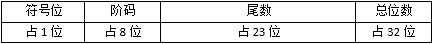
\includegraphics[width=4.51042in,height=0.45833in]{computerassets/aa2982267974c6fb0d16d1ef6ea7562a.jpeg}
4510 0000H的二进制表示为:0100 0101 0001 0000 0000 0000 0000
0000,按照浮点数格式分段后如下表所示:
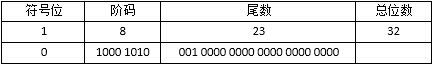
\includegraphics[width=4.51042in,height=0.67708in]{computerassets/42d8d4afe3909b90ccc7f0d4d3b29578.jpeg}
阶码为1000 1010,原码为1000 1010-0111 1111=0000
1011,对应十进制为11。(此处要注意IEEE754的移码比较特殊,差值是0111
1111)
尾数为1.001,对应的十进制为1.125。(此处也要注意,IEEE754的尾数隐藏了首位的1)。
故本题选B。
\end{solution}
\question 假定两种浮点数表示格式的位数都是32位,但格式1的阶码长,尾数短,而格式2是对格式1进行了修改,阶码减少了1位,尾数增加了1位,其他所有规定都相同,则它们可表示的数的精度和范围为
\par\fourch{两者可表示的数的范围和精度均相同}{格式1可表示的数的范围更小,但精度更高}{\textcolor{red}{格式2可表示的数的范围更小,但精度更高}}{格式1可表示的数的范围更大,但精度更高}
\begin{solution}C。
本题其实很简单,阶码越长那么能表示的最大正数和最小负数的绝对值就最大,而最大正数和最小负数其实就是表示了数的范围。故格式1可表示的数的范围更大,格式2可表示的数的范围更小。排除了A,B选项。
很明显,尾数越长,精度越高,则格式2的精度更高,格式1的精度更低。故选出正确答案C。
\end{solution}
\question 关于浮点数IEEE-754标准的规定,( )是错误的
Ⅰ.浮点数可以表示正无穷大和负无穷大两个值
Ⅱ.如果需要,也允许使用非格式化的浮点数
Ⅲ.对任何形式的浮点数都要求使用隐藏位技术
Ⅳ.对32位浮点数的阶码用移127的移码表示,尾数用原码表示
\par\twoch{仅Ⅰ、Ⅲ}{仅Ⅱ、Ⅲ}{\textcolor{red}{仅Ⅲ}}{仅Ⅰ、Ⅲ、Ⅳ}
\begin{solution}C。 Ⅰ:这个是规定的,浮点数可以表示正无穷大和负无穷大两个值;
Ⅱ:在特殊的场合当然可以使用非规格化的浮点数,只是在做加减运算时,如果不使用规格化浮点数就没有办法运算;
Ⅲ:只对规格化的浮点数才使用隐藏位技术(隐藏最高位1);
Ⅳ:浮点数IEEE-754标准规定:对32位浮点数的阶码用移127的移码表示,尾数用原码表示;
补充:为便于软件的移植,浮点数的表示格式应该有统一标准(定义)。1985年IEEE(Institute
of Electrical and Electronics
Engineers)提出了IEEE754标准。该标准规定基数为2,阶码E用移码表示,尾数M用原码表示,根据原码的规格化方法,最高数字位总是1,该标准将这个1缺省存储,使得尾数表示范围比实际存储的多一位,这样可以节省存储空间。
\end{solution}
\question 假定某计算机按字节编址,某变量x的值为\includegraphics[width=0.95833in,height=0.19792in]
% {http://texmath.koudaitiku.com/cgi-bin/mathtex.cgi?sign=847ea1\&\%5Cdpi\%7B350\%7D-\%281.25\%29*2\%5E\%7B17\%7D}
% {http://texmath.koudaitiku.com/cgi-bin/mathtex.cgi?sign=847ea1&%5Cdpi%7B350%7D-%281.25%29*2%5E%7B17%7D}
{texmath/847ea15Cdpi7B3507D281252925E7B177D}
,采用IEEE
754单精度浮点数格式表示,x的地址为F00A A000H,则在内存单元F00A
A001H中存放的内容是
\par\twoch{C9}{C4}{\textcolor{red}{20}}{00}
\begin{solution}IEEE 754标准单精度浮点数格式如下表所示:
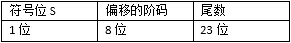
\includegraphics[width=3.03125in,height=0.44792in]{computerassets/f2a9f124b1d71a3edf9a343de8d1ad1b.jpeg}
下表给出了详细的换算过程:
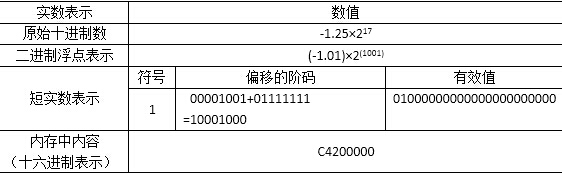
\includegraphics[width=5.85417in,height=1.81250in]{computerassets/4c5487885acb2bfc1240f0c076f1b4f6.jpeg}
由于计算机按字节(8bit)变址,该变量占32bit,占4个内存单元,内存中内容如下表所示:
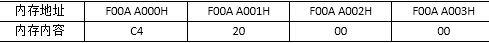
\includegraphics[width=5.09375in,height=0.44792in]{computerassets/4ff9e619662a25ffc2cdb3b30f63bc3e.jpeg}
\end{solution}
\question 一个浮点数N可以用如下方式表示:
\includegraphics[width=1.00000in,height=0.12500in]
% {http://texmath.koudaitiku.com/cgi-bin/mathtex.cgi?sign=c5cb27\&\%5Cdpi\%7B350\%7DN\%3Dm*rm\%5E\%7Be\%7D}
{texmath/847ea15Cdpi7B3507D281252925E7B177D}
,其中: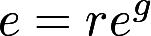
\includegraphics[width=0.55208in,height=0.12500in]{texmath/8a72405Cdpi7B3507De3Dre5E7Bg7D},
m:尾数的值,包括尾数采用的码制和数制
e:阶码的值,一般采用移码或补码,整数 rm:尾数的基 re:阶码的基
p:尾数长度,这里的p不是指尾数的二进制位数,当rm=16时,每4个二进制位表示一位尾数
q:阶码长度,由于阶码的基通常为2,因此,在一般情况下,q就是阶码部分的二进制位数
研究浮点数表示方式的主要目的是用尽量短的字长(主要是阶码字长q和尾数字长的和)实现尽可能大的表述范围和尽可能高的表数精度。根据这一目的,上述6个参数中只有3个参数是浮点数表示方式要研究的对象,它们是
\par\twoch{m、e、rm}{rm、e、rm}{re、p、q}{\textcolor{red}{rm、p、q}}
\begin{solution}D。
阶码基值re通常取为2,在目前见到的计算机系统中已经成为定论,因为在以二进制为基本计算单位的计算机系统中阶码采用其他进位制没有任何好处。所以re不是主要的研究对象。
阶码的值e通常采用整数、移码表示,只有极少数机器中采用补码表示。所以e不是主要的研究对象。
尾数m在多数计算机中用纯小数表示,只有少数机器采用整数表示,而尾数的码制有原码和补码两种,然而,尾数m的表示方法与浮点数的表述范围和表述精度基本无关。所以m也不是主要的研究对象。
综上所述,排除了三个参数,剩下的参数都是正确答案。
\end{solution}
\question 下列关于浮点数的说法中,正确的是
Ⅰ.最简单的浮点数舍入处理方法是恒置``1''法 Ⅱ.IEEE
754标准的浮点数进行乘法运算的结果肯定不需要做``左规''处理
Ⅲ.浮点数加减运算的步骤中,对阶的处理原则是小阶向大阶对齐
Ⅳ.当补码表示的尾数的最高位与尾数的符号位(数符)相同时表示规格化
Ⅴ.在浮点运算过程中如果尾数发生溢出,则应进入相应的中断处理
\par\twoch{Ⅱ、Ⅲ和Ⅴ}{\textcolor{red}{Ⅱ和Ⅲ}}{Ⅰ、Ⅱ和Ⅲ}{Ⅱ、Ⅲ、Ⅳ和Ⅴ}
\begin{solution}B。
浮点数运算的过程为对阶、尾数求和、规格化、舍入和溢出判断,本题的5个选项涉及了这5个过程。
最简单的舍入处理方法是直接截断,不进行任何其他处理(截断法),Ⅰ错误;IEEE
754标准的浮点数的尾数都是大于等于1的,所以乘法运算的结果也是大于等于1的,故不需要``左规'',Ⅱ正确;对阶的原则是小阶向大阶看齐,Ⅲ正确;当补码表示的尾数的最高位与尾数的符号位(数符)相异时表示规格化,Ⅳ错误;浮点运算过程中,尾数出现溢出并不表示真正的溢出,只有将此数右规后,再根据阶码判断是否溢出,Ⅴ错误。
\end{solution}
\question 在C语言程序中,以下程序段最终的f值为( )。 float f; f=2.5+10\^{}10;
f=f-10\^{}10;
\par\twoch{2.5}{250}{\textcolor{red}{0}}{3.5}
\begin{solution}C。 首先我们知道float类型采用IEEE754单精度浮点数格式表示,下表给出了IEEE
754标准单精度浮点数格式:
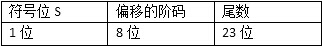
\includegraphics[width=3.36458in,height=0.48958in]{computerassets/8fda80d77778e6da3e4b1e749c1176cb.jpeg}
其中尾数隐含了一位,即尾数有24位二进制有效位数。因为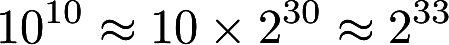
\includegraphics[width=1.60417in,height=0.16667in]{texmath/7f1bb15Cdpi7B3507D7B105E7B107D7D5Capprox105Ctimes7B25E7B307D7D5Capprox7B25E7B337D7D},在数量级大约为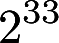
\includegraphics[width=0.21875in,height=0.15625in]{texmath/803bcc5Cdpi7B3507D25E7B337D},而2.5的数量级为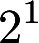
\includegraphics[width=0.14583in,height=0.15625in]{texmath/3177ee5Cdpi7B3507D25E1},因此在计算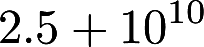
\includegraphics[width=0.72917in,height=0.16667in]
{texmath/8a2ef45Cdpi7B3507D252B7B105E7B107D7D}进行对阶时,两数阶码的差为32,也就是说,2.5的位数要右移32位,从而使得24位有效数字全部丢失,尾数变为全0。然后再与
\includegraphics[width=0.29167in,height=0.16667in]{texmath/22e2745Cdpi7B3507D105E7B107D}的位数相加,结果就是
\includegraphics[width=0.29167in,height=0.16667in]{texmath/22e2745Cdpi7B3507D105E7B107D}的尾数,因此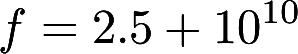
\includegraphics[width=1.07292in,height=0.18750in]
{texmath/61eb235Cdpi7B3507Df3D252B7B105E7B107D7D}
的运算结果仍为
\includegraphics[width=0.29167in,height=0.16667in]{texmath/22e2745Cdpi7B3507D105E7B107D},这样,再执行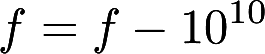
\includegraphics[width=0.94792in,height=0.18750in]{texmath/caf6545Cdpi7B3507Df3Df-7B105E7B107D7D}时结果就为0。
故本题正确答案为C。
\end{solution}
\question float型数据通常用IEEE754单精度浮点数格式表示。若编译器将float型变量x分配在一个32位浮点寄存器FR1中,且x=-8.25,则FR1的内容是(
)
\par\twoch{\textcolor{red}{C104 0000H}}{C242 0000H}{C184 0000H}{C1C2 0000H}
\begin{solution}此题着重考查IEEE
754单精度浮点数格式。只要知道格式,解题基本上就是硬套公式了。首先,将x表示成二进制,即
% \includegraphics[width=2.05208in,height=0.16667in]
% {texmath/e4857c5Cdpi7B3507D-1000013D-1.000015Ctimes7B25E7B117D7D},
{texmath/e4857c5Cdpi7B3507D-1000013D1000015Ctimes7B25E7B117D7D}
其次,应该计算阶码(不妨设为E),根据IEEE
754单精度浮点数格式有E-127=3,故E=130,换成二进制为1000
0010。最后要记住,最高位``1''是被隐藏的。 因此,根据IEEE
754格式:符号(1位)+偏移的阶码(8位)+尾数(23位),即 1+1000 0010+0000
1000 0000 0000 000 转换成十六进制:1100 0001 0000 0100 0000 0000 0000
0000,即C1040000H。 【总结】 按照IEEE
754标准,常用的浮点数有以下3种,见下表。
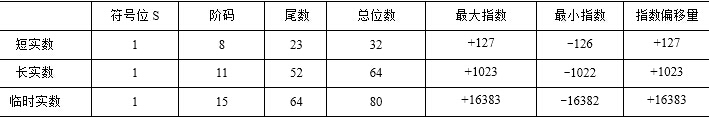
\includegraphics[width=7.38542in,height=1.22917in]{computerassets/c6f387b6aa95c2b1eb2a8d8c883630b3.jpeg}
其中,S为数符,它表示浮点数的正负,平常数符和尾数都是很``亲密''的,IEEE把它们分开了,中间插入了一个阶码,阶码中还包括阶符。在IEEE
754标准中,阶码使用移码表示,尾数用原码表示。 在IEEE
754标准中,有效位为如下形式: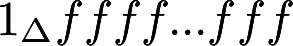
\includegraphics[width=1.05208in,height=0.15625in]{texmath/55398c5Cdpi7B3507D7B1_5CDelta7Dfffffff}
,其中,△为假想的小数点。在实际表示中,对短实数和长实数,这个整数位的1省略,称为隐藏位。
\end{solution}
\question float类型(即IEEE 754单精度浮点数格式)能表示的最大整数是( )
\par\fourch{}{}{}{\textcolor{red}{}}
\begin{solution}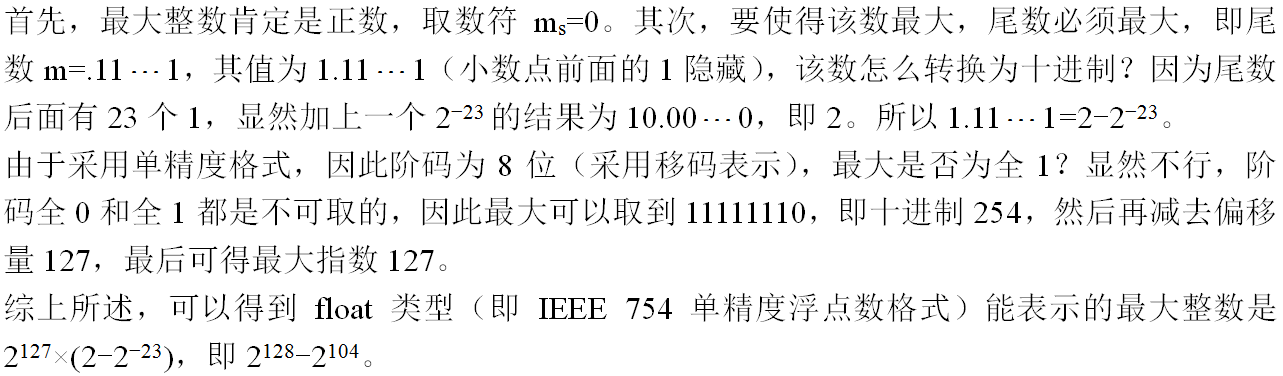
\includegraphics[width=3.46875in,height=1.02083in]{computerassets/19F28C8AD9B022A530A23C674E82250D.png}
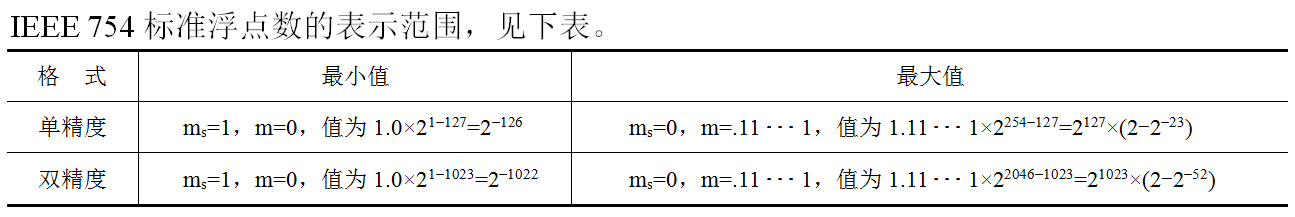
\includegraphics[width=3.46875in,height=0.58333in]{computerassets/C1F89F0A001E6310DF6522CD75904A8A.png}
\end{solution}
\question 某数采用IEEE 754单精度浮点数格式表示为C640 0000H,则该数的值是( )
\par\fourch{\textcolor{red}{}}{}{}{}
\begin{solution}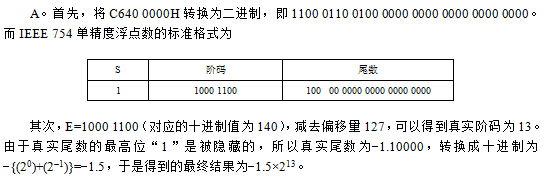
\includegraphics[width=5.67708in,height=1.87500in]{computerassets/b0063848a08156375605b5665c095cf8.jpeg}
\end{solution}
